% !TEX encoding = UTF-8 Unicode
%Präambel

%Report für große Doukumente. Dieser ist in Kapitel (\chapter{}) aufgeteilt
%\documentclass[12pt, a4paper, ngerman]{report} 

%Article für normale Doumente
\documentclass[12pt, a4paper, ngerman]{article}

%Deutsche Beschreibungen von generiertem Text (table of contents => Inhaltsverzeichnis)
\usepackage[ngerman]{babel}

%Umlaute
\usepackage[utf8]{inputenc}

%Schriftart Helvetica 
\usepackage[scaled]{helvet}

%Seitenränder
\usepackage{geometry}
%top = Abstand nach oben
%left = Abstand nach links
%right = Abstand nach rechts
%bottom= Abstand nach unten
%heapsep= Abstand zwische Kopfzeile und Text
%footskip= Abstand zwischen Text und Fußzeile
\geometry{a4paper, top=25mm, left=30mm, right=25mm, bottom=30mm, headsep=10mm, footskip=12mm}

%Farben nutzen
\usepackage{xcolor}

%Grafiken einbinden
\usepackage{graphicx}

%Zusätzliche Positionsbefehle
\usepackage{float} 

%Die Einrücktiefe bei einem neuen Absatz
\setlength{\parindent}{0pt}

%Fülltext
\usepackage{blindtext}


%Fuer Zitate	
\PassOptionsToPackage{backend=bibtex}{biblatex}
\usepackage[natbib=true,style=numeric]{biblatex}
\usepackage[babel,german=guillemets]{csquotes}
\bibliography{quellen.bib} 

% Aufnahme von \paragraph in das Inhaltsverzeichnis 
\setcounter{tocdepth}{3}  

%Nummerierung vertiefen, \paragraph kommt mit ins Inhaltsverzeichnis
\setcounter{secnumdepth}{4} 

%Feste Tabellen
\usepackage{tabulary}

%caption für nummerierte Tabellenüberschriften
%booktabs für die Steuerung von Linien
\usepackage{caption, booktabs}

%Package fuer Use Cases
\usepackage{useCases}

%Eigene Kommandos

\newcommand{\todo}[1]{\fcolorbox{red}{yellow}{ \parbox{0.75\linewidth}{#1}}} %To mark tasks can be done, but are not done 
\newcommand{\later}[1]{\fcolorbox{red}{orange}{\parbox{0.75\linewidth}{#1}}} %To mark tasks in the future. Can't be done now (e.g. missing information)
\newcommand{\checked}[1]{\fcolorbox{green}{green}{\parbox{0.75\linewidth}{#1}}} %To mark tasks, containing checked information
\newcommand{\crap}[1]{\fcolorbox{red}{red}{\parbox{0.75\linewidth}{#1}}} %To mark tasks, being absolutely bullshit

\begin{document}

\tableofcontents 
\newpage

\section{Einleitung}

\section{Use Cases}
Im Folgenden wird beschrieben, welche Use Cases das Programm in seiner Release Version bedienen kann.
\begin{figure}[htbp] 
  \centering
     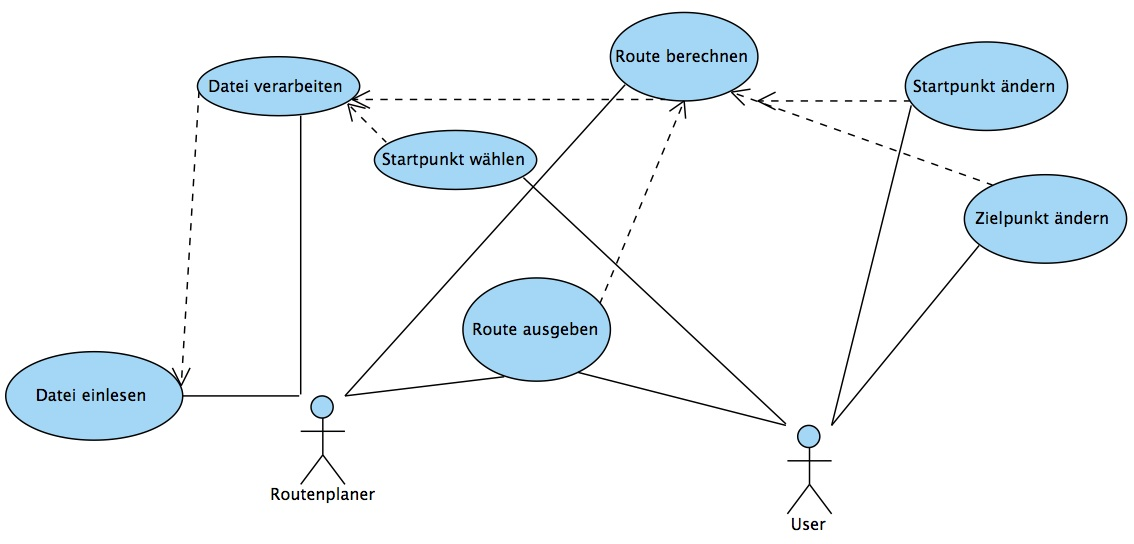
\includegraphics[width=0.9\textwidth]{Grafiken/primaryUseCases.jpg}
  \caption{Übersicht über die Use Cases}
  \label{fig:uebersichtUseCases}
\end{figure}

\subsection{Automatischer Ablauf}
\subsubsection{Datei einlesen \label{uc:DateiEinlesen}}
\begin{usecase}
	\utitle{Datei einlesen}
	\udescription{Nachdem das Programm gestartet wird, wird die csv Datei mit den Streckeninformationen eingelesen.}
	\uactor{Routenplaner}
	\utrigger{Der Start des Programms}
	\uprecondition{Eine gültige Datei mit den Streckeninformationen muss vorliegen, Der richtige Dateiname und -Pfad muss im Programm angegeben sein}
	\upostcondition{Der Inhalt der Datei befindet sich im Arbeitsspeicher}
\end{usecase}

\subsubsection{Datei verarbeiten \label{uc:DateiVerarbeiten}}
\begin{usecase}
	\utitle{Datei verarbeiten}
	\udescription{Aus der bereits eingelesenen Datei werden Objekte erstellt.}
	\uactor{Routenplaner}
	\utrigger{Die Verarbeitung Use Case \ref{uc:DateiEinlesen} ist abgeschlossen}
	\uprecondition{Use Case \ref{uc:DateiEinlesen}}
	\upostcondition{Die primäre Funktionalität des Routenplaners steht dem User zur Verfügung}
\end{usecase}

\subsection{Abläufe, die vom User angestoßen werden}
\subsubsection{Startpunkt wählen \label{uc:StartpunktWaehlen}}
\begin{usecase}
	\utitle{Startpunkt wählen}
	\udescription{Der User wählt den Startpunkt der Routenberechnung aus}
	\uactor{User}
	\uprecondition{Use case \ref{uc:DateiVerarbeiten}}
	\upostcondition{Die Route wird berechnet}
\end{usecase}
\end{document}